\chapter{Bit Manipulation}\label{ch:bit_manipulation}
\section{Thinking in Bit Manipulation}
\subsection{Encoding for Integers}
\subsubsection{Encoding for Unsigned Integers}
Given a {\color{blue}{bit vector}} of {\color{blue}{$w$}} bits, {\color{blue}{$\vec{x} = \left[x_{w-1}, x_{w-2}, \dots, x_0\right]$}}, we can interpret it as an {\color{blue}{unsigned integer}}:
\begin{equation}
{\color{blue}{B2U_w\left(\vec{x}\right) = \sum_{i=0}^{w-1}x_i2^i}}
\end{equation}

For example, assume $w = 4$, we have:
\begin{align*}
B2U_4([0001]) &= 0 \cdot 2^3 + 0 \cdot 2^2 + 0 \cdot 2^1 + 1 \cdot 2^0 = 0 + 0 + 0 + 1 = 1 \\
B2U_4([0101]) &= 0 \cdot 2^3 + 1 \cdot 2^2 + 0 \cdot 2^1 + 1 \cdot 2^0 = 0 + 4 + 0 + 1 = 5 \\
B2U_4([1011]) &= 1 \cdot 2^3 + 0 \cdot 2^2 + 1 \cdot 2^1 + 1 \cdot 2^0 = 8 + 0 + 2 + 1 = 11 \\
B2U_4([1111]) &= 1 \cdot 2^3 + 1 \cdot 2^2 + 1 \cdot 2^1 + 1 \cdot 2^0 = 8 + 4 + 2 + 1 = 15
\end{align*}\mbox{}

Let us consider the {\color{blue}{range}} of values that can be represented using $w$ bits. The least value is given by bit vector $\left[0, 0, \dots, 0\right]$ having integer value {\color{blue}{$UMin_w = 0$}}, and the greatest value is given by bit vector $\left[1, 1, \dots, 1\right]$ having integer value {\color{blue}{$UMax_w = \sum_{i=0}^{w-1}2^i = w^2 - 1$}}. Using the $4$-bit case as an example, we have $UMax_4 = B2U_4([1111]) = 2^4 - 1= 15$. Thus, the function $B2U_w$ can be defined as a mapping {\color{blue}{$B2U_w : \left\{0, 1\right\}^w \rightarrow \left\{0, \dots, 2^{w-1}\right\}$}}.\\

The unsigned binary representation has the important property that every number between $0$ and $2^w - 1$ has a unique encoding as a $w$-bit value. For example, there is only one representation of decimal value $11$ as an unsigned, $4$-bit number, namely $[1, 0, 1, 1]$. This property is captured in mathematical terms by stating that function {\color{blue}{$B2U_w$ is a bijection}} -- it associates a unique value to each bit vector of length $w$; conversely, each integer between $0$ and $2^w - 1$ has a unique binary representation as a bit vector of length $w$.

\subsubsection{Encoding For Signed Integers - Two's Complement}
For many applications, we wish to represent {\color{blue}{negative values}} as well. The most common computer representation of signed numbers is known as {\color{blue}{two’s-complement}} form. This is defined by interpreting the most significant bit of the word to have negative weight. We express this interpretation as a function $B2T_w$:
\begin{equation}
{\color{blue}{B2T_w\left(\vec{x}\right) = -x_{w-1}2^{w-1} + \sum_{i=0}^{w-2}x_i2^i}}
\end{equation}
The most significant bit $x_{w-1}$ is also called the {\color{blue}{sign bit}}. Its “weight” is $-2^{w-1}$ , the negation of its weight in an unsigned representation. When the sign bit is set to $1$, the represented value is negative, and when set to $0$ the value is nonnegative.\\

For example, assume $w = 4$, we have:
\begin{align*}
B2T_4([0001]) &= -0 \cdot 2^3 + 0 \cdot 2^2 + 0 \cdot 2^1 + 1 \cdot 2^0 = 0 + 0 + 0 + 1 = 1 \\
B2T_4([0101]) &= -0 \cdot 2^3 + 1 \cdot 2^2 + 0 \cdot 2^1 + 1 \cdot 2^0 = 0 + 4 + 0 + 1 = 5 \\
B2T_4([1011]) &= -1 \cdot 2^3 + 0 \cdot 2^2 + 1 \cdot 2^1 + 1 \cdot 2^0 = -8 + 0 + 2 + 1 = -5 \\
B2T_4([1111]) &= -1 \cdot 2^3 + 1 \cdot 2^2 + 1 \cdot 2^1 + 1 \cdot 2^0 = -8 + 4 + 2 + 1 = -1
\end{align*}\mbox{}

Let us consider the {\color{blue}{range}} of values that can be represented as a $w$-bit two’scomplement number. The least representable value is given by bit vector {\color{blue}{$[1, 0, \dots, 0]$}} (set the bit with negative weight, but clear all others), having integer value {\color{blue}{$TMin_w  = -2^{w-1}$}}. The greatest value is given by bit vector {\color{blue}{$[0, 1, \dots, 1] $}} (clear the bit with negative weight, but set all others), having integer value {\color{blue}{$TMax_w=\sum_{i=0}^{w-2}2^i = 2^{w-1} - 1$}}. Using the $4$-bit case as an example, we have $TMin_4 = B2T_4 ([1000]) = -2^3 = -8$, and $TMax_4 = B2T_4 ([0111]) = 2^2 + 2^1 + 2^0 = 4 + 2 + 1 = 7$.\\

We can see that $B2T_w$ is a mapping of bit patterns of length $w$ to numbers between $TMin_w$ and $TMax_w$, written as {\color{blue}{$B2T_w: \left\{0, 1\right\}^w \rightarrow \left\{-2^{w-1} ,\dots, 2^{w-1} - 1\right\}$}}. As we saw with the unsigned representation, every number within the representable range has a unique encoding as a $w$-bit two’s-complement number. In mathematical terms, we say that the function {\color{blue}{$B2T_w$ is a bijection}}—it associates a unique value to each bit vector of length w; conversely, each integer between $-2^{w-1}$ and $2^{w-1} - 1$ has a unique binary representation as a bit vector of length $w$.

\subsection{Conversions Between Signed and Unsigned}
When converting between {\color{blue}{signed}} and {\color{blue}{unsigned}} integers of the {\color{blue}{same word size}}, the {\color{blue}{bit patterns}} remain the same and the {\color{blue}{values}} may change.\\

\subsubsection*{Two's complement to Unsigned}
\begin{equation}
{\color{blue}{T2U_w(x) = B2U_w\left(T2B_w(x)\right) = 
\begin{cases} 
x + 2^w, & x \leq 0 \\
x, & x \geq 0 
\end{cases}}}
\end{equation}
\begin{figure}[H]
\centering
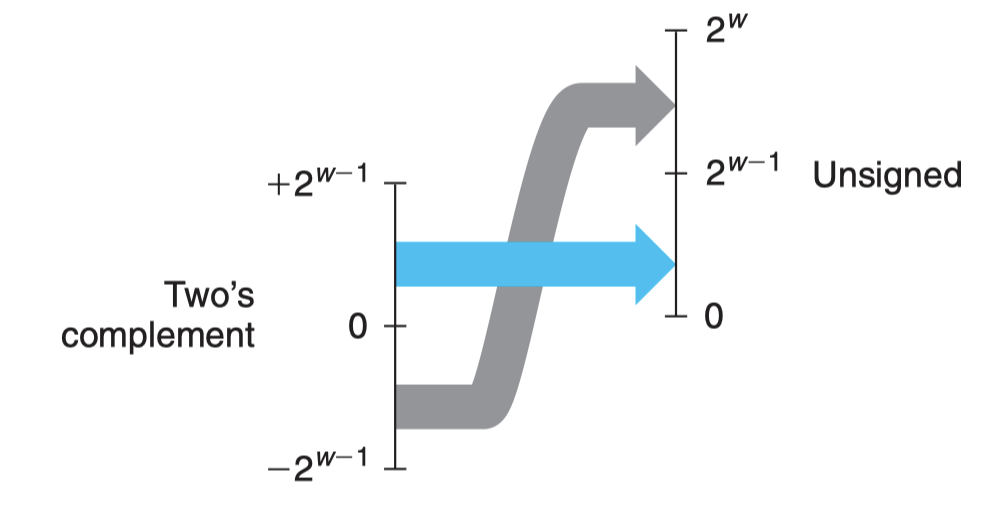
\includegraphics[width=0.4\linewidth]{images/t2u}
\label{fig:t2u}
\end{figure}

\subsubsection*{Unsigned to Two's complement}
\begin{equation}
{\color{blue}{U2T_w(u) = B2T_w\left(U2B_w(x)\right) = 
\begin{cases} 
u, & u < 2^w-1 \\
u - 2^w, & u \geq 2^w-1 
\end{cases}}}
\end{equation}
\begin{figure}[H]
\centering
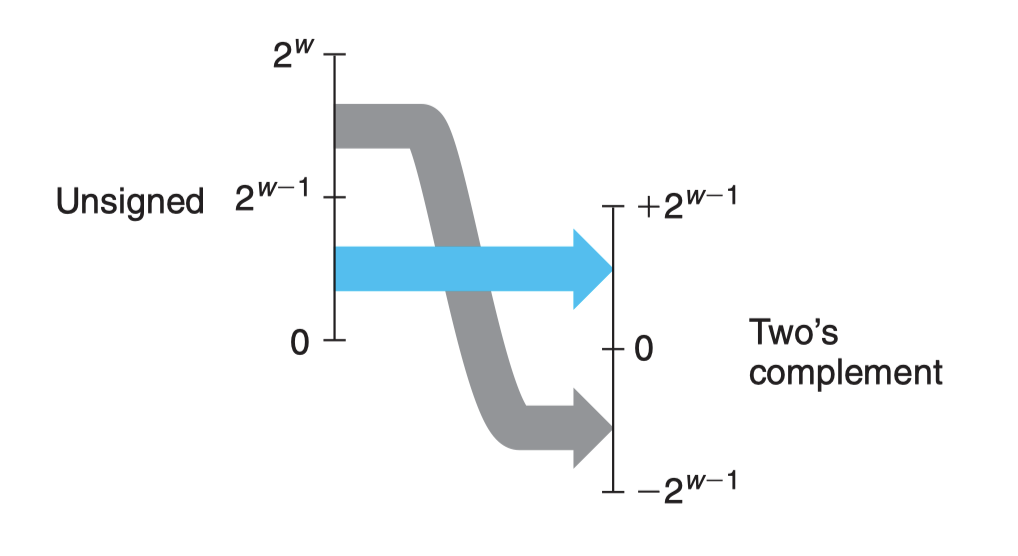
\includegraphics[width=0.4\linewidth]{images/u2t}
\label{fig:u2t}
\end{figure}

\subsection{Expanding the Bit Representation of a Number}
To convert an {\color{blue}{unsigned}} integer to a {\color{blue}{larger data type}}, we can simply add leading zeros to the representation; this operation is known as {\color{blue}{zero extension}}.\\

To convert a {\color{blue}{two’s complement}} integer to a {\color{blue}{larger data type}}, the rule is to perform a {\color{blue}{sign extension}}, adding copies of the {\color{blue}{most significant bit}} to the representation.\\

Note that extending a number never alters its value. (The proof is ignored.)

\subsection{Truncating the Bit Representation of a Number}
When truncating a {\color{blue}{$w$-bit}} number {\color{blue}{$x = [x_{w-1} , x_{w-2} ,\dots, x_0]$}} to a {\color{blue}{$k$-bit}} number, we {\color{blue}{drop the high-order $w - k$ bits}}, giving a bit vector {\color{blue}{$x' = [x_{k-1}, x_{k-2}, \dots, x_0]$}}.\\

Note that truncating a number can alter its value. (Obvious.)

\subsection{Bitwise Logical Operators in C++}
The {\color{blue}{bitwise logical operators}} ({\colorbox{CodeBackground}{\lstinline|&, \|, ~, ^, <<, >>|}}) are applied to {\color{blue}{integral types}},  e.g., {\colorbox{CodeBackground}{\lstinline|char|}}, {\colorbox{CodeBackground}{\lstinline|short|}}, {\colorbox{CodeBackground}{\lstinline|int|}}, {\colorbox{CodeBackground}{\lstinline|long|}}, {\colorbox{CodeBackground}{\lstinline|long long|}} and their {\color{blue}{unsigned counterparts}}.
 
\subsubsection{Bitwise AND {\colorbox{CodeBackground}{\lstinline|&|}}}

\subsubsection{Bitwise OR {\colorbox{CodeBackground}{\lstinline|\||}}}

\subsubsection{Bitwise XOR {\colorbox{CodeBackground}{\lstinline|^|}}}
\begin{lstlisting}
x ^ x = 0
x ^ 0 = x
a ^ b = b ^ a
a ^ (b ^ c) = (a ^ b) ^ c
\end{lstlisting}

\subsubsection{Bitwise Complement {\colorbox{CodeBackground}{\lstinline|\~|}}}

\subsubsection{Left Shift {\colorbox{CodeBackground}{\lstinline|<<|}}}
In terms of {\color{blue}{bit patterns}}, {\color{blue}{left shifts}} {\colorbox{CodeBackground}{\lstinline|<<|}} are consistent across {\color{blue}{signed}} and {\color{blue}{unsigned}} integers, which is to introduce zeros into the {\color{blue}{least significant bit (LSB)}}. Any bits that are shifted beyond the range of the {\color{blue}{most significant bit (MSB)}} are discarded.\\

For {\color{blue}{unsigned integers}}, the interpretation is straightforward. The left shift operation is equivalent to multiplying the number by $2^n$ (where $n$ is the number of positions shifted), assuming no overflow occurs. If the value after the shift exceeds the maximum representable value for the data type, the resulting behavior is well-defined; the excess bits are simply discarded, often resulting in a wrapped-around value.\\

For {\color{blue}{signed integers}}, the situation is more complex due to the presence of the {\color{blue}{sign bit}}. When left shifting, if any $1$ bits are shifted into the sign bit position, or if the sign bit is shifted out and changes the perceived sign of the number, the behavior is undefined according to the C++ standard. This means that the compiler is not required to handle this situation in any particular way, and the resulting value could be different depending on the compiler and the machine.

\subsubsection{Right Shift {\colorbox{CodeBackground}{\lstinline|>>|}}}
{\color{blue}{Right shifts}} indeed behave differently on {\color{blue}{signed}} and {\color{blue}{unsigned}} integers due to how they handle the {\color{blue}{sign bit}}.\\

For {\color{blue}{unsigned integers}}, right shifts are straightforward: bits are moved to the right, and the leftmost bits are filled with zeros. This operation is equivalent to dividing the number by $2^n$ is the number of positions shifted, and any remainder is discarded. There's no ambiguity because there is no sign bit to consider, making the right shift operation for unsigned integers well-defined and predictable.\\

For {\color{blue}{signed integers}}, right shifts are more complex because they must account for the {\color{blue}{sign bit}}. In C++, right shifts on signed integers typically perform an "{\color{blue}{arithmetic shift}}" where the sign bit is replicated to the leftmost bits. This preserves the sign of the number: if it's positive, zeros are shifted in (just like with unsigned integers), but if it's negative, ones are shifted in to keep the number negative. This behavior can differ between systems and compilers, although arithmetic shifting is the most common.

\section{LC 0231 - Power of Two}\label{lc0231}
Given an integer {\colorbox{CodeBackground}{\lstinline|n|}}, return {\colorbox{CodeBackground}{\lstinline|true|}} if it is a power of {\colorbox{CodeBackground}{\lstinline|2|}}. Otherwise, return {\colorbox{CodeBackground}{\lstinline|false|}}.\\

Examples:
\begin{itemize}
\item {\colorbox{CodeBackground}{\lstinline|n = 1 -> true|}}
\item {\colorbox{CodeBackground}{\lstinline|n = 16 --> true|}}
\item {\colorbox{CodeBackground}{\lstinline|n = 3 --> false|}}
\end{itemize}

\subsection*{Solution - Bit Manipulation}\label{solution:lc0231_bit_manipulation}
A number is a power of two if it has exactly one bit set in its binary representation. For example, {\colorbox{CodeBackground}{\lstinline|4|}} is {\colorbox{CodeBackground}{\lstinline|100|}} in binary, and {\colorbox{CodeBackground}{\lstinline|16|}} is {\colorbox{CodeBackground}{\lstinline|10000|}} in binary. If you subtract {\colorbox{CodeBackground}{\lstinline|1|}} from such number:
\begin{itemize}
\item all the bits less than the single set bit will become {\colorbox{CodeBackground}{\lstinline|1|}};
\item the set bit will become {\colorbox{CodeBackground}{\lstinline|0|}};
\item all the bits greater than the single set bit will keep the same;
\end{itemize}
If you bitwise AND this result with the original number, you should get {\colorbox{CodeBackground}{\lstinline|0|}}.
\begin{lstlisting}
bool isPowerOfTwo(int n) {
  if (n <= 0) { return false; }
  return (n & (n - 1)) == 0;
}
\end{lstlisting}

\subsection*{Other Solutions}
\begin{itemize}
\item \hyperref[solution:lc0231_simulation_iterative]{Simulation (Iterative)}
\item \hyperref[solution:lc0231_simulation_recursion]{Simulation (Recursion)}
%\item \hyperref[solution:lc0231_bit_manipulation]{Bit Manipulation}
\end{itemize}

\subsection*{Related}
\begin{itemize}
\item \hyperref[lc0231]{LC 0231 - Power of Two}
\item \hyperref[lc0342]{LC 0342 - Power of Four}
\end{itemize}

\section{LC 0342 - Power of Four}\label{lc0342}
Given an integer {\colorbox{CodeBackground}{\lstinline|n|}}, return {\colorbox{CodeBackground}{\lstinline|true|}} if it is a power of {\colorbox{CodeBackground}{\lstinline|4|}}. Otherwise, return {\colorbox{CodeBackground}{\lstinline|false|}}.\\

Examples:
\begin{itemize}
\item {\colorbox{CodeBackground}{\lstinline|n = 16 --> true|}}
\item {\colorbox{CodeBackground}{\lstinline|n = 5 --> false|}}
\item {\colorbox{CodeBackground}{\lstinline|n = 1 --> true|}}
\end{itemize}

\subsection*{Solution - Bit Manipulation}\label{solution:lc0342_bit_manipulation}
{\colorbox{CodeBackground}{\lstinline|n|}} is power of {\colorbox{CodeBackground}{\lstinline|four|}} if and only if:
\begin{itemize}
\item {\colorbox{CodeBackground}{\lstinline|n|}} is power of {\colorbox{CodeBackground}{\lstinline|2|}};
\item and {\colorbox{CodeBackground}{\lstinline|1|}} is at one of the odd positions;
\end{itemize}
\begin{lstlisting}
bool isPowerOfFour(int n) {
  if (n <= 0) { return false; }
  return (n & (n - 1)) == 0 && (n & 0xAAAAAAAA) == 0;
}
\end{lstlisting}

\subsection*{Other Solutions}
\begin{itemize}
\item \hyperref[solution:lc0342_simulation_iterative]{Simulation (Iterative)}
\item \hyperref[solution:lc0342_simulation_recursion]{Simulation (Recursion)}
%\item \hyperref[solution:lc0342_bit_manipulation]{Bit Manipulation}
\end{itemize}

\subsection*{Related}
\begin{itemize}
\item \hyperref[lc0231]{LC 0231 - Power of Two}
\item \hyperref[lc0342]{LC 0342 - Power of Four}
\end{itemize}

\section{LC 0268 - Missing Number}
Given a \ul{non-empty} array {\colorbox{CodeBackground}{\lstinline|nums|}} containing {\colorbox{CodeBackground}{\lstinline|n|}} distinct numbers in the range {\colorbox{CodeBackground}{\lstinline|[0, n]|}}, return the only number in the range that is missing from the array.\\

Examples:
\begin{itemize}
\item {\colorbox{CodeBackground}{\lstinline|nums = [3,0,1] --> 2|}}
\item {\colorbox{CodeBackground}{\lstinline|nums = [0,1] --> 2|}}
\item {\colorbox{CodeBackground}{\lstinline|nums = [9,6,4,2,3,5,7,0,1] --> 8|}}
\end{itemize}

\subsection*{Solution - Bit manipulation}\label{solution:lc0268_bit_manipulation}
\begin{lstlisting}
int missingNumber(const std::vector<int>& nums) {
  int xor_sum = 0;
  for (int i = 0; i <= nums.size(); ++i) { xor_sum ^= i; }
  for (int num : nums) { xor_sum ^= num; }
  return xor_sum;
}
\end{lstlisting}

\subsection*{Other Solutions}
\begin{itemize}
\item \hyperref[solution:lc0268_mathematical_formula]{Mathematical Formula}
\end{itemize}

\section{LC 0389 - Find the Difference}
You are given two strings {\colorbox{CodeBackground}{\lstinline|s|}} and {\colorbox{CodeBackground}{\lstinline|t|}}.\\

String {\colorbox{CodeBackground}{\lstinline|t|}} is generated by random shuffling string {\colorbox{CodeBackground}{\lstinline|s|}} and then add one more letter at a random position.\\

Return the letter that was added to {\colorbox{CodeBackground}{\lstinline|t|}}.\\

Examples:
\begin{itemize}
\item {\colorbox{CodeBackground}{\lstinline|s = "abcd", t = "abcde" --> "e"|}}
\item {\colorbox{CodeBackground}{\lstinline|s = "", t = "y" --> "y"|}}
\end{itemize}

\subsection*{Solution - Bit Manipulation}
\begin{lstlisting}
char findTheDifference(std::string s, std::string t) {
  char diff = 0;
  for (char c : s) diff ^= c;
  for (char c : t) diff ^= c;
  return diff;
}
\end{lstlisting}

\section{LC 0136 - Single Number}
Given a \ul{non-empty} array of integers {\colorbox{CodeBackground}{\lstinline|nums|}}, every element appears twice except for one. Find that single one.\\

Examples:
\begin{itemize}
\item {\colorbox{CodeBackground}{\lstinline|nums = [2,2,1] --> 1|}}
\item {\colorbox{CodeBackground}{\lstinline|nums = [4,1,2,1,2] --> 4|}}
\item {\colorbox{CodeBackground}{\lstinline|nums = [1] --> 1|}}
\end{itemize}

\subsection*{Solution - Bit Manipulation}
\begin{lstlisting}
int singleNumber(std::vector<int>& nums) {
  int single = 0;
  for (int num : nums) { single ^= num; }
  return single;
}
\end{lstlisting}

\section{LC 0137 - Single Number II}
Given a \ul{non-empty} array of integers {\colorbox{CodeBackground}{\lstinline|nums|}}, every element appears three times except for one. Find that single one.\\

Examples:
\begin{itemize}
\item {\colorbox{CodeBackground}{\lstinline|nums = [2,2,3,2] --> 3|}}
\item {\colorbox{CodeBackground}{\lstinline|nums = [0,1,0,1,0,1,99] --> 99|}}
\end{itemize}

\subsection*{Solution - Bit Manipulation}
The idea is to count how many times each bit appears in the numbers. Since each number appears three times, except for one, if we sum the bits in each position for all numbers and then take modulo {\colorbox{CodeBackground}{\lstinline|3|}}, the result must be either {\colorbox{CodeBackground}{\lstinline|0|}} or the bit of the unique number.
\begin{lstlisting}
int singleNumber(std::vector<int>& nums) {
  int single = 0;
  for (int i = 0; i < 32; i++) {
    int digit_cnt = 0;
    for (int num : nums) {
      if ((num >> i) & 1) { ++digit_cnt; }
    }
    if (digit_cnt % 3) { single |= (1 << i); }
  }
  return single;
}
\end{lstlisting}

\section{LC 0029 - Divide Two Integers}
Given two integers {\colorbox{CodeBackground}{\lstinline|dividend|}} and {\colorbox{CodeBackground}{\lstinline|divisor|}} ({\colorbox{CodeBackground}{\lstinline|divisor != 0|}}), divide two integers without using \ul{multiplication}, \ul{division}, and \ul{mod} operator.\\

The integer division should \ul{truncate toward zero}, which means losing its \ul{fractional part}. For example, {\colorbox{CodeBackground}{\lstinline|8.345|}} would be truncated to {\colorbox{CodeBackground}{\lstinline|8|}}, and {\colorbox{CodeBackground}{\lstinline|-2.7335|}} would be truncated to {\colorbox{CodeBackground}{\lstinline|-2|}}.\\

Return the \ul{quotient} after dividing {\colorbox{CodeBackground}{\lstinline|dividend|}} by {\colorbox{CodeBackground}{\lstinline|divisor|}}.\\

Note: Assume we are dealing with an environment that could only store integers within the {\colorbox{CodeBackground}{\lstinline|32|}}-bit signed integer range:  {\colorbox{CodeBackground}{\lstinline|[-2^31, 2^31 - 1]|}}.  For this problem, if the quotient is strictly greater than {\colorbox{CodeBackground}{\lstinline|2^31 - 1|}}, then return {\colorbox{CodeBackground}{\lstinline|2^31 - 1,|}} and if the quotient is strictly less than {\colorbox{CodeBackground}{\lstinline|-2^31|}}, then return {\colorbox{CodeBackground}{\lstinline|-2^31|}}.

\subsection*{Solution - Bit Manipulation}\label{solution:lc0029_bit_manipulation}
\begin{lstlisting}
int divide(int dividend, int divisor) {
  // edge case - overflow
  if (dividend == std::numeric_limits<int>::min() && divisor == -1) {
    return std::numeric_limits<int>::max();
  }
  int sign = ((dividend < 0) ^ (divisor < 0)) ? -1 : 1;
  // use long type to avoid overflow
  long cur_dividend = std::abs(static_cast<long>(dividend));
  long cur_divisor = std::abs(static_cast<long>(divisor));
  long quotient = 0;
  while (cur_dividend >= cur_divisor) {
    long tmp = cur_divisor;
    long multiple = 1;
    while (cur_dividend >= (tmp << 1)) {
      tmp <<= 1;
      multiple <<= 1;
    }
    cur_dividend -= tmp;
    quotient += multiple;
  }
  return sign * quotient;
}
\end{lstlisting}

\subsection*{Other Solutions}
\begin{itemize}
\item \hyperref[solution:lc0029_repeated_substraction]{*Repeated Subtraction (Time Limit Exceeded)}
%\item \hyperref[solution:lc0029_bit_manipulation]{Bit Manipulation}
\end{itemize}

\section{LC 0190 - Reverse Bits}
Reverse bits of a given {\colorbox{CodeBackground}{\lstinline|32|}} bits \ul{unsigned integer}.\\

Examples:
\begin{itemize}
\item {\colorbox{CodeBackground}{\lstinline|n = 00000010100101000001111010011100 --> 00111001011110000010100101000000|}}
\item {\colorbox{CodeBackground}{\lstinline|n = 11111111111111111111111111111101 --> 10111111111111111111111111111111|}}
\end{itemize}

\subsection*{Solution - Bit Manipulation}
\begin{lstlisting}
uint32_t reverseBits(uint32_t n) {
  uint32_t result = 0;
  for (int i = 0; i < 32; i++) {
    uint32_t bit = (n >> i) & 1;
    result |= (bit << (31 - i));
  }
  return result;
}
\end{lstlisting}

\section{LC 0191 - Number of 1 Bits (Hamming Weight)}
Write a function that takes the binary representation of an \ul{unsigned integer} and returns the number of {\colorbox{CodeBackground}{\lstinline|1|}} bits it has.\\

Examples:
\begin{itemize}
\item {\colorbox{CodeBackground}{\lstinline|n = 00000000000000000000000000001011 --> 3|}}
\item {\colorbox{CodeBackground}{\lstinline|n = 00000000000000000000000010000000 --> 0|}}
\item {\colorbox{CodeBackground}{\lstinline|n = 11111111111111111111111111111101 --> 31|}}
\end{itemize}

\subsection*{Solution - Bit Manipulation}
\begin{lstlisting}
int hammingWeight(uint32_t n) {
  int cnt = 0;
  while (n != 0) {
    cnt += n & 1;
    n = n >> 1;
  }
  return cnt;
}
\end{lstlisting}

\section{LC 0201 - Bitwise AND of Numbers Range}
Given two integers {\colorbox{CodeBackground}{\lstinline|left >= 0|}} and {\colorbox{CodeBackground}{\lstinline|right >= 0|}}, return the bitwise AND of all numbers in range {\colorbox{CodeBackground}{\lstinline|[left, right]|}}.\\

Examples:
\begin{itemize}
\item {\colorbox{CodeBackground}{\lstinline|left = 5, right = 7 --> 4 (5 & 6 & 7 = 4)|}}
\item {\colorbox{CodeBackground}{\lstinline|left = 0, right = 0 --> 0|}}
\item {\colorbox{CodeBackground}{\lstinline|left = 1, right = 2147483647 --> 0|}}
\end{itemize}

\subsection*{Solution - Bit Manipulation}
\begin{lstlisting}
int rangeBitwiseAnd(int left, int right) {
  int shift = 0;
  // find common prefix of numbers in range [left, right]
  while (left < right) {
    left >>= 1;
    right >>= 1;
    ++shift;
  }
  // shift prefix back to the original position
  return left << shift;
}
\end{lstlisting}

\section{LC 0338 - Counting Bits}
Given an integer {\colorbox{CodeBackground}{\lstinline|n|}}, return an array {\colorbox{CodeBackground}{\lstinline|ans|}} of length {\colorbox{CodeBackground}{\lstinline|n + 1|}} such that for each {\colorbox{CodeBackground}{\lstinline|i|}} ({\colorbox{CodeBackground}{\lstinline|0 <= i <= n|}}), {\colorbox{CodeBackground}{\lstinline|ans[i]|}} is the number of {\colorbox{CodeBackground}{\lstinline|1|}}s in the binary representation of {\colorbox{CodeBackground}{\lstinline|i|}}.\\

Examples:
\begin{itemize}
\item {\colorbox{CodeBackground}{\lstinline|n = 2 --> [0,1,1]|}}
\item {\colorbox{CodeBackground}{\lstinline|n = 5 --> [0,1,1,2,1,2]|}}
\end{itemize}

\subsection*{Solution 1 - DP}
\begin{lstlisting}
std::vector<int> countBits(int n) {
  std::vector<int> cnt(n + 1);
  cnt[0] = 0;
  for (int i = 1; i <= n; ++i) {
    if (i % 2 == 0) {
      cnt[i] = cnt[i / 2];
    } else {
      cnt[i] = cnt[i / 2] + 1;
    }
  }
  return cnt;
}
\end{lstlisting}

\subsection*{Solution 1 - DP, Optimized}
\begin{lstlisting}
std::vector<int> countBits(int n) {
  std::vector<int> cnt(n + 1);
  cnt[0] = 0;
  for (int i = 1; i <= n; ++i) { cnt[i] = cnt[i >> 1] + (i & 1); }
  return cnt;
}
\end{lstlisting}

\section{LC 0405 - Convert a Number to Hexadecimal}\label{lc0405}
Given an integer {\colorbox{CodeBackground}{\lstinline|num|}}, return a string representing its \ul{hexadecimal representation}. For negative integers, two’s complement method is used.\\

All the letters in the answer string should be lowercase characters, and there should not be any leading zeros in the answer except for the zero itself.\\

Examples:
\begin{itemize}
\item {\colorbox{CodeBackground}{\lstinline|num = 26 --> "1a"|}}
\item {\colorbox{CodeBackground}{\lstinline|num = -1 --> "ffffffff"|}}
\end{itemize}

\subsection*{Solution - Bit Manipulation}
\begin{lstlisting}
std::string toHex(int num) {
  if (num == 0) { return "0"; }
  std::string hex = "0123456789abcdef";
  std::string hex_str = "";
  // process the number for 32 bits, skip leading zeros
  for (int i = 0; num != 0 && i < 8; ++i) {
    int dec = num & 0xf;
    hex_str = hex[dec] + hex_str;
    num >>= 4;
  }
  return hex_str;
}
\end{lstlisting}

\subsection*{Related}
\begin{itemize}
\item \hyperref[lc0504]{LC 0504 - Base 7}
\item \hyperref[lc0405]{LC 0405 - Convert a Number to Hexadecimal}
\end{itemize}

\section{LC 0461 - Hamming Distance}
Given two integers {\colorbox{CodeBackground}{\lstinline|x|}} and {\colorbox{CodeBackground}{\lstinline|y|}}, return the \ul{Hamming Distance} between them.\\

The \ul{Hamming Distance} between two integers is the number of positions at which the corresponding bits are different.\\

Examples:
\begin{itemize}
\item {\colorbox{CodeBackground}{\lstinline|x = 1, y = 4 --> 2|}}
\item {\colorbox{CodeBackground}{\lstinline|x = 3, y = 1 --> 1|}}
\end{itemize}

\subsection*{Solution - Bit Manipulation}
\begin{lstlisting}
int hammingDistance(int x, int y) {
  int xor_val = x ^ y;
  int distance = 0;
  while (xor_val) {
    distance += xor_val & 1;
    xor_val >>= 1;
  }
  return distance;
}
\end{lstlisting}

\section{LC 0287 - Find the Duplicate Number}
Given an array of integers {\colorbox{CodeBackground}{\lstinline|nums|}} containing {\colorbox{CodeBackground}{\lstinline|n + 1|}} integers where each integer is in the range {\colorbox{CodeBackground}{\lstinline|[1, n]|}}. There is only one duplicate number in {\colorbox{CodeBackground}{\lstinline|nums|}}, find and return it.\\


Examples:
\begin{itemize}
\item {\colorbox{CodeBackground}{\lstinline|nums = [1,3,4,2,2] --> 2|}}
\item {\colorbox{CodeBackground}{\lstinline|nums = [3,1,3,4,2] --> 3|}}
\end{itemize}

\subsection*{Solution - Bit Manipulation}
TODO

\section{LC 0397 - Integer Replacement}
Given a \ul{positive integer} {\colorbox{CodeBackground}{\lstinline|n|}}, you can apply one of the following operations:
\begin{enumerate}
\item If {\colorbox{CodeBackground}{\lstinline|n|}} is even, replace {\colorbox{CodeBackground}{\lstinline|n|}} with {\colorbox{CodeBackground}{\lstinline|n / 2|}}.
\item If {\colorbox{CodeBackground}{\lstinline|n|}} is odd, replace {\colorbox{CodeBackground}{\lstinline|n|}} with either {\colorbox{CodeBackground}{\lstinline|n + 1|}} or{\colorbox{CodeBackground}{\lstinline| n - 1|}}.
\end{enumerate}
Return the minimum number of operations needed for {\colorbox{CodeBackground}{\lstinline|n|}} to become {\colorbox{CodeBackground}{\lstinline|1|}}.\\

Examples:
\begin{itemize}
\item {\colorbox{CodeBackground}{\lstinline|n = 8 --> 3 (8 -> 4 -> 2 -> 1)|}}
\item {\colorbox{CodeBackground}{\lstinline|n = 7 --> 4 (7 -> 8 -> 4 -> 2 -> 1 or 7 -> 6 -> 3 -> 2 -> 1)|}}
\end{itemize}

\subsection*{Solution - Bit Manipulation}
TODO

\section{LC 0421 - Maximum XOR of Two Numbers in an Array}
Given an integer array {\colorbox{CodeBackground}{\lstinline|nums|}}, return the maximum result of {\colorbox{CodeBackground}{\lstinline|nums[i] XOR nums[j]|}}, where {\colorbox{CodeBackground}{\lstinline|0 <= i <= j < n|}}.\\

Examples:
\begin{itemize}
\item {\colorbox{CodeBackground}{\lstinline|nums = [3,10,5,25,2,8] --> 28|}}
\item {\colorbox{CodeBackground}{\lstinline|nums = [14,70,53,83,49,91,36,80,92,51,66,70] --> 127|}}
\end{itemize}

\subsection*{Solution - Bit Manipulation}
TODO

\section{LC 0465 - Optimal Account Balancing}
You are given an array of transactions {\colorbox{CodeBackground}{\lstinline|transactions|}} where {\colorbox{CodeBackground}{\lstinline|transactions[i] = [from_i, to_i, amount_i]|}} indicates that the person with {\colorbox{CodeBackground}{\lstinline|ID = from_i|}} gave {\colorbox{CodeBackground}{\lstinline|amount_i|}} to the person with {\colorbox{CodeBackground}{\lstinline|ID = to_i|}}.\\

Return the minimum number of transactions required to settle the debt.\\

Examples:
\begin{itemize}
\item {\colorbox{CodeBackground}{\lstinline|transactions = [[0,1,10],[2,0,5]] --> 2|}}
\item {\colorbox{CodeBackground}{\lstinline|transactions = [[0,1,10],[1,0,1],[1,2,5],[2,0,5]] --> 1|}}
\end{itemize}

\subsection*{Solution - Bit Manipulation}
TODO

\section{LC 0526 - Beautiful Arrangement}
Suppose you have n integers labeled {\colorbox{CodeBackground}{\lstinline|1|}} through {\colorbox{CodeBackground}{\lstinline|n|}}. A permutation of those {\colorbox{CodeBackground}{\lstinline|n|}} integers {\colorbox{CodeBackground}{\lstinline|perm|}} ({\colorbox{CodeBackground}{\lstinline|1|}}-indexed) is considered a \ul{beautiful arrangement} if for every {\colorbox{CodeBackground}{\lstinline|i|}} ({\colorbox{CodeBackground}{\lstinline|1 <= i <= n|}}), either of the following is true:
\begin{itemize}
\item perm[i] is divisible by i.
\item i is divisible by perm[i].
\end{itemize}
Given an integer {\colorbox{CodeBackground}{\lstinline|n|}}, return the number of the beautiful arrangements that you can construct.\\

Examples:
\begin{itemize}
\item {\colorbox{CodeBackground}{\lstinline|n = 2 --> 2|}}
\item {\colorbox{CodeBackground}{\lstinline|n = 1 --> 1|}}
\end{itemize}

\subsection*{Solution - Bit Manipulation}
TODO

\section{LC 0645 - Set Mismatch}
You have a set of integers {\colorbox{CodeBackground}{\lstinline|s|}}, which originally contains all the numbers from {\colorbox{CodeBackground}{\lstinline|1|}} to {\colorbox{CodeBackground}{\lstinline|n|}}. Unfortunately, due to some error, one of the numbers in {\colorbox{CodeBackground}{\lstinline|s|}} got duplicated to another number in the set, which results in repetition of one number and loss of another number.\\

You are given an integer array {\colorbox{CodeBackground}{\lstinline|nums|}} representing the data status of this set after the error.\\

Find the number that occurs twice and the number that is missing and return them in the form of an array.\\

Examples:
\begin{itemize}
\item {\colorbox{CodeBackground}{\lstinline|nums = [1,2,2,4] -- [2,3]|}}
\item {\colorbox{CodeBackground}{\lstinline|nums = [1,1] --> [1,2]|}}
\end{itemize}

\subsection*{Solution - Bit Manipulation}
TODO

\section{LC 0779 - K-th Symbol in Grammar}
We build a table of {\colorbox{CodeBackground}{\lstinline|n|}} rows ({\colorbox{CodeBackground}{\lstinline|1|}}-indexed). We start by writing {\colorbox{CodeBackground}{\lstinline|0|}} in the {\colorbox{CodeBackground}{\lstinline|1|}}st row. Now in every subsequent row, we look at the previous row and replace each occurrence of {\colorbox{CodeBackground}{\lstinline|0|}} with {\colorbox{CodeBackground}{\lstinline|01|}}, and each occurrence of {\colorbox{CodeBackground}{\lstinline|1|}} with {\colorbox{CodeBackground}{\lstinline|10|}}. For example, for {\colorbox{CodeBackground}{\lstinline|n = 3|}}, the {\colorbox{CodeBackground}{\lstinline|1|}}st row is {\colorbox{CodeBackground}{\lstinline|0|}}, the {\colorbox{CodeBackground}{\lstinline|2|}}nd row is {\colorbox{CodeBackground}{\lstinline|01|}}, and the {\colorbox{CodeBackground}{\lstinline|3|}}rd row is {\colorbox{CodeBackground}{\lstinline|0110|}}.\\

Given two integer {\colorbox{CodeBackground}{\lstinline|n|}} and {\colorbox{CodeBackground}{\lstinline|k|}}, return the {\colorbox{CodeBackground}{\lstinline|k|}}th ({\colorbox{CodeBackground}{\lstinline|1|}}-indexed) symbol in the {\colorbox{CodeBackground}{\lstinline|n|}}th row of a table of {\colorbox{CodeBackground}{\lstinline|n|}} rows.\\

Examples:
\begin{itemize}
\item {\colorbox{CodeBackground}{\lstinline|n = 1, k = 1 --> 0|}}
\item {\colorbox{CodeBackground}{\lstinline|n = 2, k = 1 --> 0|}}
\item {\colorbox{CodeBackground}{\lstinline|n = 2, k = 2 --> 1|}}
\end{itemize}

\subsection*{Solution - Bit Manipulation}
TODO

\section{LC 0898 - Bitwise ORs of Subarrays}
Given an integer array {\colorbox{CodeBackground}{\lstinline|arr|}}, return the number of distinct bitwise ORs of all the non-empty subarrays of {\colorbox{CodeBackground}{\lstinline|arr|}}.\\

The bitwise OR of a subarray is the bitwise OR of each integer in the subarray. The bitwise OR of a subarray of one integer is that integer.\\

Examples:
\begin{itemize}
\item {\colorbox{CodeBackground}{\lstinline|arr = [0] --> 1|}}
\item {{\colorbox{CodeBackground}{\lstinline|arr = [1,1,2] --> 3|}}}
\item {\colorbox{CodeBackground}{\lstinline|arr = [1,2,4] --> 6|}}
\end{itemize}

\subsection*{Solution - Bit Manipulation}
TODO

\section{LC 1009 - Complement of Base 10 Integer}
The complement of an integer is the integer you get when you flip all the {\colorbox{CodeBackground}{\lstinline|0|}}'s to {\colorbox{CodeBackground}{\lstinline|1|}}'s and all the {\colorbox{CodeBackground}{\lstinline|1|}}'s to {\colorbox{CodeBackground}{\lstinline|0|}}'s in its binary representation. For example, The integer {\colorbox{CodeBackground}{\lstinline|5|}} is {\colorbox{CodeBackground}{\lstinline|"101"|}} in binary and its complement is {\colorbox{CodeBackground}{\lstinline|"010"|}} which is the integer {\colorbox{CodeBackground}{\lstinline|2|}}.\\

Given an integer {\colorbox{CodeBackground}{\lstinline|n|}}, return its complement.\\

Examples:
\begin{itemize}
\item {\colorbox{CodeBackground}{\lstinline|n = 5 --> 2|}}
\item {\colorbox{CodeBackground}{\lstinline|n = 7 --> 0|}}
\item {\colorbox{CodeBackground}{\lstinline|n = 10 --> 5|}}
\end{itemize}

\subsection*{Solution - Bit Manipulation}
TODO

\section{LC 1356 - Sort Integers by The Number of 1 Bits}
You are given an integer array {\colorbox{CodeBackground}{\lstinline|arr|}}. Sort the integers in the array in ascending order by the number of {\colorbox{CodeBackground}{\lstinline|1|}}'s in their binary representation and in case of two or more integers have the same number of {\colorbox{CodeBackground}{\lstinline|1|}}'s you have to sort them in ascending order.\\

Return the array after sorting it.\\

Examples:
\begin{itemize}
\item {\colorbox{CodeBackground}{\lstinline|arr = [0,1,2,3,4,5,6,7,8] --> [0,1,2,4,8,3,5,6,7]|}}
\item {\colorbox{CodeBackground}{\lstinline|arr = [1024,512,256,128,64,32,16,8,4,2,1] --> [1,2,4,8,16,32,64,128,256,512,1024]|}}
\end{itemize}

\subsection*{Solution - Bit Manipulation}
TODO

\section{LC 1707 - Maximum XOR With an Element From Array}
You are given an array {\colorbox{CodeBackground}{\lstinline|nums|}} consisting of non-negative integers. You are also given a {\colorbox{CodeBackground}{\lstinline|queries|}} array, where {\colorbox{CodeBackground}{\lstinline|queries[i] = [x_i, m_i]|}}.\\

The answer to the {\colorbox{CodeBackground}{\lstinline|i|}}th query is the maximum bitwise {\colorbox{CodeBackground}{\lstinline|XOR|}} value of {\colorbox{CodeBackground}{\lstinline|x_i|}} and any element of {\colorbox{CodeBackground}{\lstinline|nums|}} that does not exceed {\colorbox{CodeBackground}{\lstinline|m_i|}}. In other words, the answer is {\colorbox{CodeBackground}{\lstinline|max(nums[j] XOR x_i)|}} for all {\colorbox{CodeBackground}{\lstinline|j|}} such that {\colorbox{CodeBackground}{\lstinline|nums[j] <= m_i|}}. If all elements in {\colorbox{CodeBackground}{\lstinline|nums|}} are larger than {\colorbox{CodeBackground}{\lstinline|m_i|}}, then the answer is {\colorbox{CodeBackground}{\lstinline|-1|}}.\\

Return an integer array {\colorbox{CodeBackground}{\lstinline|answer|}} where {\colorbox{CodeBackground}{\lstinline|answer.length == queries.length|}} and {\colorbox{CodeBackground}{\lstinline|answer[i]|}} is the answer to the {\colorbox{CodeBackground}{\lstinline|i|}}th query.\\

Examples:
\begin{itemize}
\item {\colorbox{CodeBackground}{\lstinline|nums = [0,1,2,3,4], queries = [[3,1],[1,3],[5,6]] --> [3,3,7]|}}
\textit{{\colorbox{CodeBackground}{\lstinline|nums = [5,2,4,6,6,3], queries = [[12,4],[8,1],[6,3]] --> [15,-1,5]|}}}
\end{itemize}

\subsection*{Solution - Bit Manipulation}
TODO